% article example for classicthesis.sty
\documentclass[10pt,a4paper]{article} % KOMA-Script article scrartcl
\usepackage{lipsum}     %lorem ipsum text
\usepackage{titlesec}   %Section settings
\usepackage{titling}    %Title settings
\usepackage[margin=10em]{geometry}  %Adjusting margins
\usepackage{setspace}
\usepackage{listings}
\usepackage{amsmath}    %Display equations options
\usepackage{amssymb}    %More symbols
\usepackage{xcolor}     %Color settings
\usepackage{pagecolor}
\usepackage{mdframed}
\usepackage[spanish]{babel}
\usepackage[utf8]{inputenc}
\usepackage{longtable}
\usepackage{multicol}
\usepackage{graphicx}
\graphicspath{ {./Images/} }
\setlength{\columnsep}{1cm}

% ====| color de la pagina y del fondo |==== %
\pagecolor{black}
\color{white}



\begin{document}
    %========================{TITLE}====================%
    \title{\rmfamily\normalfont\spacedallcaps{ Notas clase 2 distancias }}
    \author{\spacedlowsmallcaps{Rodrigo Castillo}}
    \date{\today} 
    
    \maketitle
     

     % ====| Loguito |==== %
    
\includegraphics[width=0.1\linewidth]{negro_cara.png}
    %=======================NOTES GOES HERE===================%
    empezamos con la tarea de luisa
    \section{Distancia}

        \subsection{distacia euclideana}
            la distancia euclideana es la distancia clásica, el teorema de
            pitágoras y está dada como :
            \begin{equation}
                D(a,b) = \sqrt{x _{1}^{2} + x_2 ^{2} + ... + x_p ^{2}    } 
            \end{equation}
            pero en estadística la distancia euclideana no es la mas apropiada
            pues cada componente se pondera de la misma forma, esto aplica en
            longitudes pero no en variables estadísticas

        \subsection{distancia estadística}
            si hay medidas que tienen variaciones aleatorias hay que ponderar
            unas medidas con mayor peso y otras con menor peso , esto se hace
            así : 
            distancia estadística:
            % ====| seria bueno poner la grafica de las suposiciones |==== %
            % ====| tambien sería severo poner las suposiciones      |==== %
            % ====| también sería severo poner las observaciones |==== %
            \begin{equation}
               estandarizacion  = x*_1 =  \frac{x_1}{\sqrt{s _{11} } }
            \end{equation}
            
            \\ el truco es estandarizar
            \\ una vez estandarizamos calculamos la ditancia euclideana
                
            \begin{equation}
                D(O,P) =  \sqrt{(\frac{x_1}{s _{11} })^{2} + (\frac{x_2}{s _{22} } )^{2}  } 
            \end{equation}

            % ====| poner imagen de la elipse |==== %
            distancia entre 2 puntos :
            % ====| PONER LA DISTANCIA ENTRE DOS PUNTOS  |==== %
            \subsection{distancia estadística en p dimensiones}
                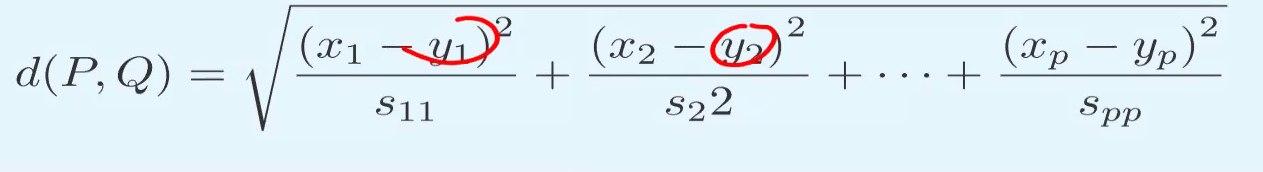
\includegraphics[width=0.8\linewidth]{distancia_p_dimensiones.png}
                consideraciones:
                \begin{enumerate}
                    \item {si s _{11} = s _{22} = ... =  s _{pp} 
                    \\ es mejor usar la distancia euclideana   } 
                \end{enumerate}
                cuando hay dependencias la distancia no es la mejor
            \subsection{distancia estadistica con correlaciones:}
                \begin{equation}
                    D(o,p) = \sqrt{ \frac{xgorro _{2} ^{2}} {s _{11} } + \frac{xgorro _{2} ^{2}  }{ s _{22} } } 
                \end{equation}
                
                esto es si hay dependencias , si no hay dependencias volvemos a
                la distancia anterior
            \subsection{generalizacion de la distancia estadística con correlaciones}
                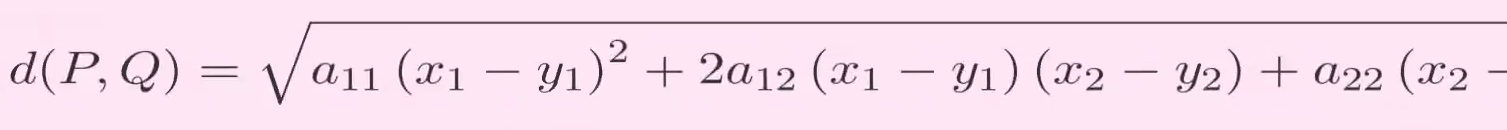
\includegraphics[width=0.6\linewidth]{distancia_estadistica_corr.png}
            \subsection{propiedades de las distancias}
            \begin{itemize}
                \item {D(P,Q) = D(Q,P)} 
                \item {D(p,q) != 0 si p!=q} 
                \item {desigualdad triangular} 
            \end{itemize}	
            
            \section{repaso de algebra vectorial}
                \subsection{vectores:}
                    las cosas clasicas de vectores de algebra lieanl
                \subsection{independencia lineal}
                    un conjunto de vectores $ x_1 , x_2 , ... , x_k  $ es
                    linealmente indepentiendes si existen constantes $ c_1 ,
                    c_2 , ... , c_n  $ tales que     
                    \begin{equation}
                        c_1 \times x_1 + c_2 \times x_2 + ... + c_k \times x_k  = 0
                    \end{equation}
                    formas para saber que un conjunto de vectores son
                    linealmente independientes 
                \subsection{proyeccion vectorial}
                    se tiene un vector y un vector y , se proyecta el vector x sobre y
                    \begin{equation}
                        Proy = \frac{x'y}{L_y} \times \frac{1}{L_y}y
                    \end{equation}
                \subsection{matrices}
                    \begin{equation}
                        transA = A'
                    \end{equation}
                \subsection{teorema importante}
                    a es invertible sii las columas de A son linealmente independientes
                
                \subsection{vectores y valores propios}
                    son fundamentales en la estadística 
                    \\ un valor propio se caracteriza por $ A_x = lamda x  $  
                
        
    







    %=======================NOTES ENDS HERE===================%
    
    % bib stuff
    \nocite{*}
    \addtocontents{toc}{\protect\vspace{\beforebibskip}}
    \addcontentsline{toc}{section}{\refname}    
    \bibliographystyle{plain}
    \bibliography{../Bibliography}
\end{document}
